% !TeX encoding = UTF-8
% !TeX program = XeLaTeX
% !TeX spellcheck = en_US

% Author : Shlw
% Description : TikZ Assignment
\documentclass{standalone}

\usepackage{tikz}
\usetikzlibrary{automata}

\begin{document}

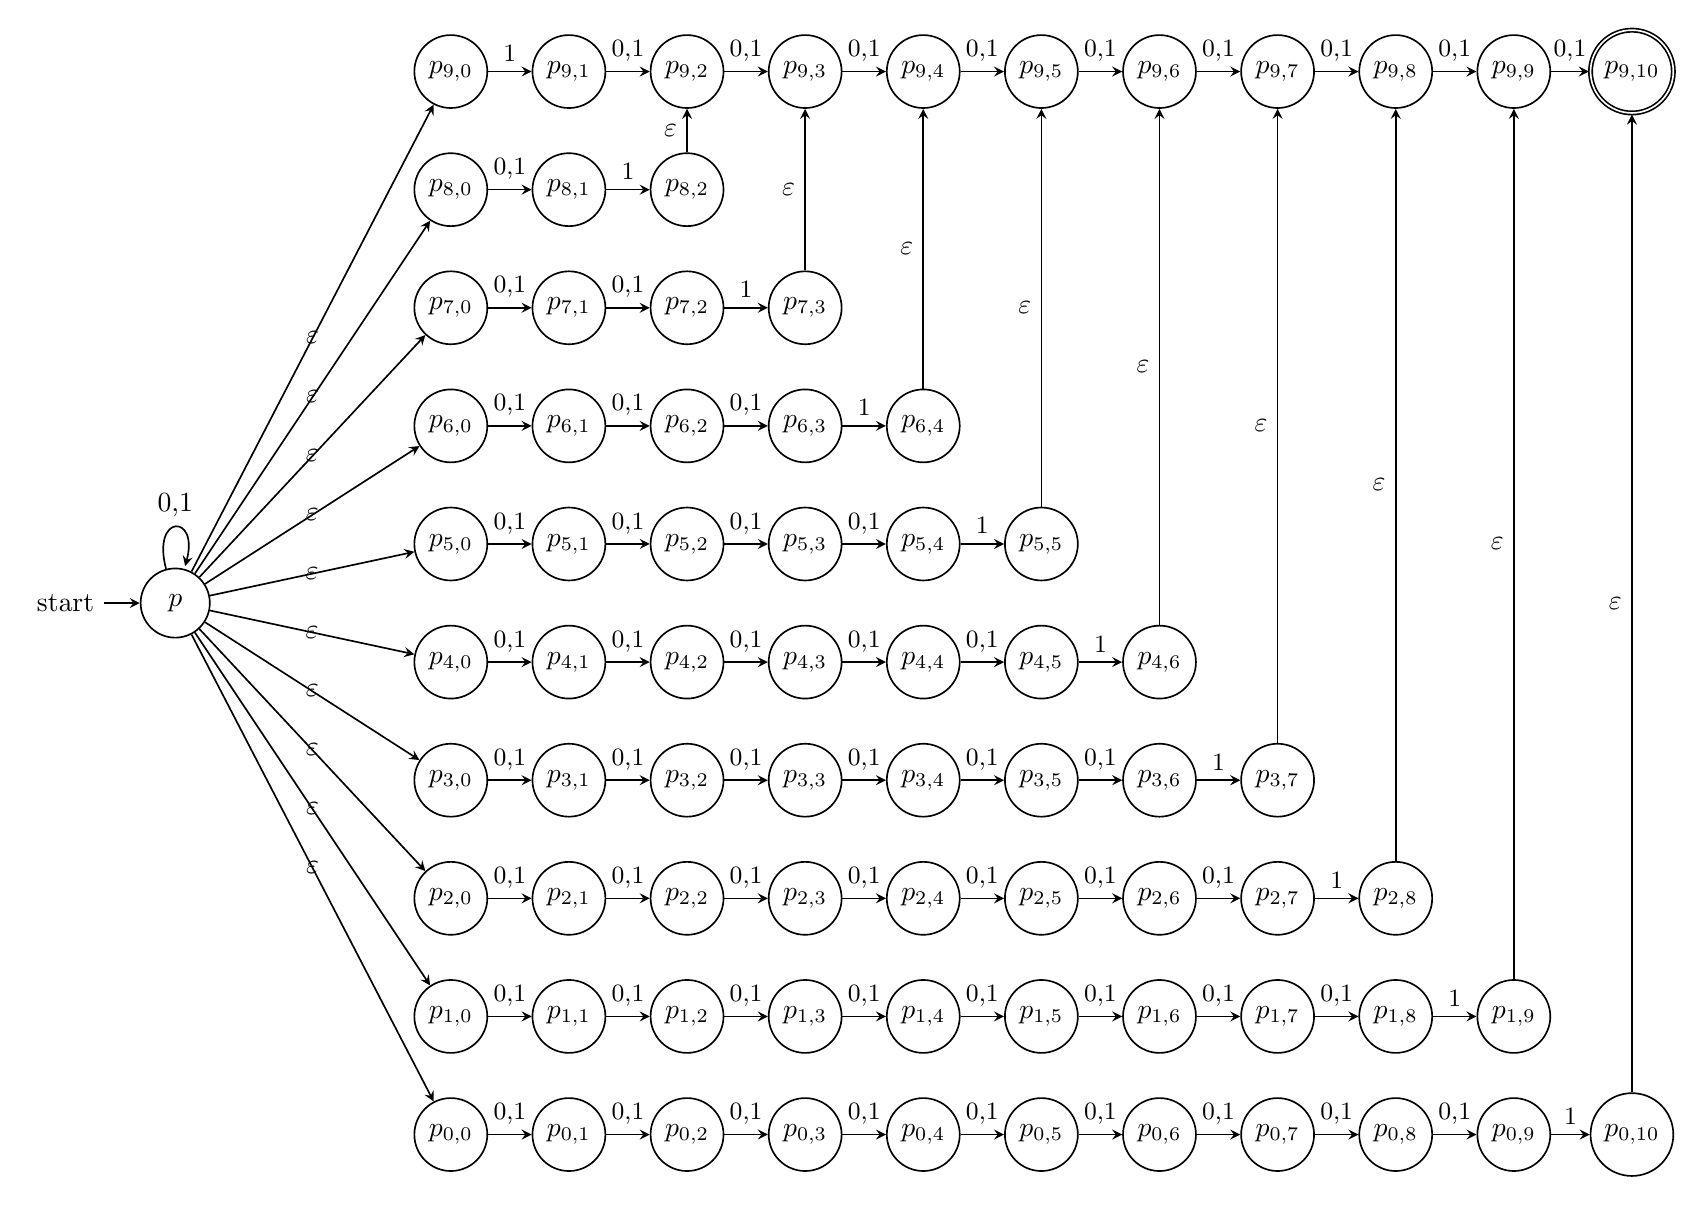
\begin{tikzpicture}[>=stealth,semithick,node distance=1.5cm,auto]

\node[state,initial left] (p) at (-3.5,4.5*1.5) {$p$};
\path[->] (p) edge [loop above] node {0,1} ();

\foreach \x [evaluate=\x as \y using \x*1.5,remember=\x as \pre] in {0,...,10}{
    \ifnum \x=10
        \node[state,accepting] (p-9-\x) at (\y,9*1.5) {$p_{9,\x}$};
    \else
        \node[state] (p-9-\x) at (\y,9*1.5) {$p_{9,\x}$};
    \fi

    \ifnum \x>1
        \path[->] (p-9-\pre) edge node {\small 0,1} (p-9-\x);
    \else
        \ifnum \x=1
            \path[->] (p-9-\pre) edge node {\small 1} (p-9-\x);
        \fi
    \fi
}

\foreach \y [evaluate=\y as \z using 9-\y] in {0,...,8}
    \foreach \x [remember=\x as \pre] in {0,...,10}{
        \node[state] (p-\y-\x) at (\x*1.5,\y*1.5) {$p_{\y,\x}$};

        \ifnum \x>0
            \ifnum \x>\z
                \path[->] (p-\y-\pre) edge node {\small 1} (p-\y-\x);
            \else
                \path[->] (p-\y-\pre) edge node {\small 0,1} (p-\y-\x);
            \fi
        \fi
        
        \ifnum \x>\z
            \path[->] (p-\y-\x) edge node {$\varepsilon$} (p-9-\x);
            \breakforeach
        \fi
    }

\foreach \x in {0,...,9}
    \path[->] (p) edge node [above,yshift=-2mm] {$\varepsilon$} (p-\x-0);
    
\end{tikzpicture}

\end{document}
